\section{Experiments} 
We have implemented our method in python \footnote{The entirety of the code, networks and datasets utilized in our evaluation are available on https://github.com/digumx/unified-merges.}, utilizing the NumPy library for linear algebra operations and the SciPy library for an implementation of \hcluster. We have used a linkage-matrix-based data structure similar to the one used in SciPy to store the tree and have precomputed and cached several operations that may need to be repeated every refinement iteration. This allows us to quickly perform the merge and split operations and calculate the scores (Section \ref{s:refinement}), without having to do (relatively)
expensive tree traversal operations in each iteration of the abstraction refinement loop.

Using this implementation, we have performed a set of experiments demonstrating the effectiveness of our abstraction technique for verification of neural network queries on the \acasxu set of networks, using both the original safety properties from \cite{reluplex} and the $\epsilon$-robustness properties introduced in \cite{cegar-nn}. To do so, we set up a \cegar loop (Section \ref{s:abs-ref-fw}) using our abstraction technique, using the \neuralsat solver as the underlying solver to dispatch the verification queries on \abs. We compare our abstraction framework with the existing \cegar framework proposed in \cite{cegar-nn} \footnote{We have used a faithful re-implementation of this framework that follows exactly the procedure in the paper, with the only two distinctions being that we are using a two-class classification as seen in \cite{chauhan2022efficiently,liu2022abstraction,10.1145/3644387},
and that the call to verify the \abs obtained in each iteration is sent to an instance of the \neuralsat solver as opposed to \marabou. } setting a timeout of 200 seconds for each instance in the benchmark and for both our technique and the existing work. The experiments were run on a machine running on Intel(R) Core(TM) i7-6700 CPU with 8 CPUs running at 3.40GHz, having 16 GB of RAM, and running Ubuntu 22.04 LTS.


If the \abs produced has multiple neurons with the exact same set of incoming edges in the same layer, these neurons compute the same function and are redundant. Therefore, as an added optimization step in our method, we safely \textit{re-merge} them by summing up the weights of the outgoing edges. Note that this does not change the behavior of \abs.

\begin{table}
    \vspace*{-0.25cm}
    \centering
        \begin{tabular}{ |c|c|c|c|c| }
        \hline
        Method                   & No. Safe    & No. Unsafe & No. Timeout & Average Size \\ 
        \hline
        Ours                     &   121       & 43         & 16          &  335.3\\
        Existing \cite{cegar-nn} &   118       & 43         & 19          &  536.0\\
        \hline                                                                
        \end{tabular}
        \caption{Summary of \acasxu on original safety properties }
        \label{t:acas-verif}
    \vspace{-1.5cm}
\end{table}
\begin{table}
    \centering
    \begin{tabular}{ |c|c|c| }
    \hline
    Method                   & Percentage Verified  & Average Size \\ 
    \hline
    Ours                     &   100\%              &  27.9\\
    Existing \cite{cegar-nn} &   100\%              &  31.5\\
    \hline                                                                
    \end{tabular}
    \caption{Summary of \acasxu on robustness properties }
    \label{t:acas-verif-robustness}
    %\vspace{-1cm}
    \vspace*{-0.75cm}
\end{table}


Tables \ref{t:acas-verif} and \ref{t:acas-verif-robustness} summarizes the
results on these benchmarks. We
find that using our framework, we are able to perform better than the existing
\cegar approach on the original safety properties, verifying
more networks to be safe, while we do not loose performance on the robustness
properties. 

\begin{wrapfigure}{r}{0.5\textwidth}
    \vspace*{-0.5cm}
    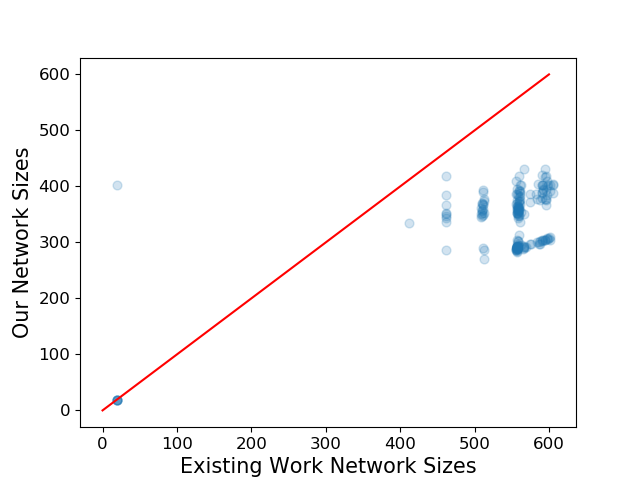
\includegraphics[scale=0.4]{scatter-cegar-our-nerualsat-diag-new.png}
    \vspace{0.15cm}
    \caption{Scatter plot of network sizes produced by our framework vs existing
    work \cite{cegar-nn} on \acasxu }
    \label{f:scatter-netsizes}
    \vspace*{-0.5cm}
\end{wrapfigure}

For each framework, we collected the final \abs at the end of the \cegar iterations, for which either the property can be proved to be safe, or the solver is able to find an actual counterexample, or the solver times out. Figure \ref{f:scatter-netsizes} shows a scatter plot comparing the sizes of these final \abs obtained by our framework and by existing work \cite{cegar-nn} for each instance in the benchmark.
A point below the red diagonal line represents an instance for which we obtain a smaller final \abs than the existing work; therefore, points below the line represent instances for which we perform better.
The average sizes of these \abs over all instances are reported in the `Average Size' columns in tables \ref{t:acas-verif} and \ref{t:acas-verif-robustness}.

It is apparent from Figure \ref{f:scatter-netsizes}, Table \ref{t:acas-verif}, and Table \ref{t:acas-verif-robustness} that, compared to the existing techniques, we explore smaller \abs that are effective at proving or disproving the property in question. This shows that using semantic information to guide the CEGAR process can effectively find more efficient abstractions than the existing technique.


Note that in our experiments, we found that the time taken by both our CEGAR approach and the existing CEGAR approach \cite{cegar-nn} was more than what the \neuralsat solver takes for the \acasxu benchmarks. However, while we would expect the solver call times to exponentially scale with network size, the overheads from the abstraction procedure will not scale exponentially. Thus, for larger and larger benchmarks, being able to find smaller \abs will produce a significant difference in times. Furthermore, we believe that a verified \abs is useful beyond verifying a single property - it may be used for other related queries or may be useful as a safely deployable compressed network.


Additionally, we find that the final solver times on the \abs are actually comparable with the times obtained on the original un-abstracted \cnc. In general, it has been observed both by our experiments and in \cite{cegar-nn} that the effort needed to verify a network is dependent on more than just network size. In fact, in \cite{cegar-nn}, they are able to achieve smaller solver times on larger networks.
While it is true that in general the worst-case performance of neural network solvers will almost certainly remain exponential in the size of the network \cite{reluplex}, other factors on which the performance of neural network solvers may depend remain an interesting direction of future work.


